\section{Prospetto economico}
Vengono mostrati i prospetti economici per ciascuna fase di progetto, divisi per ruolo. Le fasi di \AR e \AD non sono a carico del committente.

\subsection{\AR}
Nella fase di \AR le ore sono suddivise nel modo seguente:
\begin{table}[H]
	\centering
	\begin{tabular}{|c|c|c|}
		\hline
		\textbf{Ruolo} &
		\textbf{Ore} &
		\textbf{Costo} \\
		\hline
		Responsabile & 30 & 900\\
		\hline
		Amministratore & 29 & 580\\
		\hline
		Analista & 90 & 2250\\
		\hline
		Progettista & 0 & 0 \\
		\hline
		Programmatore & 0 & 0 \\
		\hline
		Verificatore & 40 & 600\\
		\hline
		\textbf{Totale} & \textbf{189} & \textbf{4330} \\
		\hline
	\end{tabular}
	\caption{Costo per ruolo, fase di \AR}
\end{table}

I seguenti grafici mostrano visivamente come abbiano influiranno i ruoli per ore e costi nella fase di \AR.
\begin{figure}[H]
	\centering
	\scalebox{0.6}{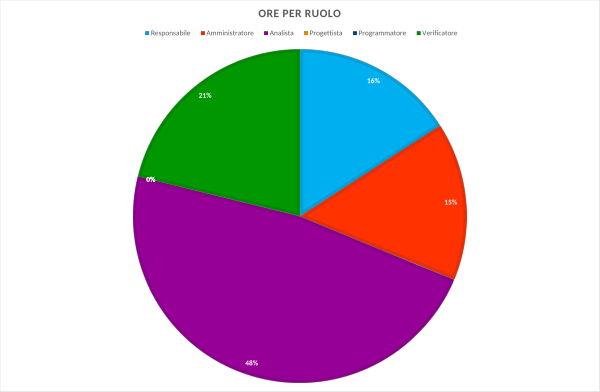
\includegraphics{img_peconomico/AA_OR.png}}
	\caption{Ore per ruoli, fase di \AR}
\end{figure}
\begin{figure}[H]
	\centering
	\scalebox{0.6}{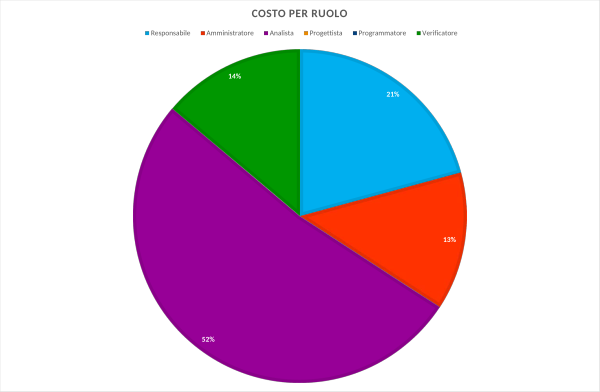
\includegraphics{img_peconomico/AA_CR.png}}
	\caption{Costi per ruolo, fase di \AR}
\end{figure}

\subsection{\AD}
Nella fase di \AD le ore sono suddivise nel modo seguente:
\begin{table}[H]
	\centering
	\begin{tabular}{|c|c|c|}
		\hline
		\textbf{Ruolo} &
		\textbf{Ore} &
		\textbf{Costo} \\
		\hline
		Responsabile & 1 & 30\\
		\hline
		Amministratore & 1 & 20\\
		\hline
		Analista & 15 & 375\\
		\hline
		Progettista & 0 & 0 \\
		\hline
		Programmatore & 0 & 0 \\
		\hline
		Verificatore & 4 & 60\\
		\hline
		\textbf{Totale} & \textbf{21} & \textbf{485} \\
		\hline
	\end{tabular}
	\caption{Costo per ruolo, fase di \AD}
\end{table}

I seguenti grafici mostrano visivamente come abbiano influiranno i ruoli per ore e costi nella fase di \AD.
\begin{figure}[H]
	\centering
	\scalebox{0.6}{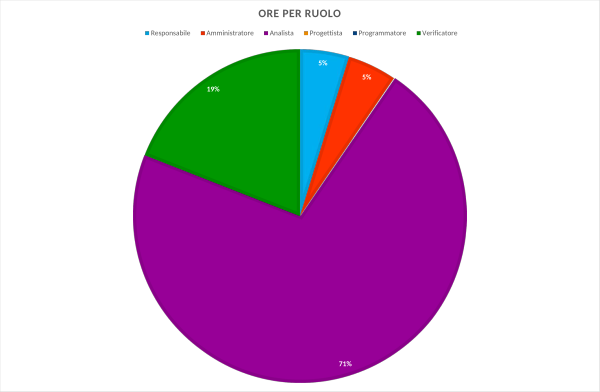
\includegraphics{img_peconomico/AD_OR.png}}
	\caption{Ore per ruoli, fase di \AD}
\end{figure}
\begin{figure}[H]
	\centering
	\scalebox{0.6}{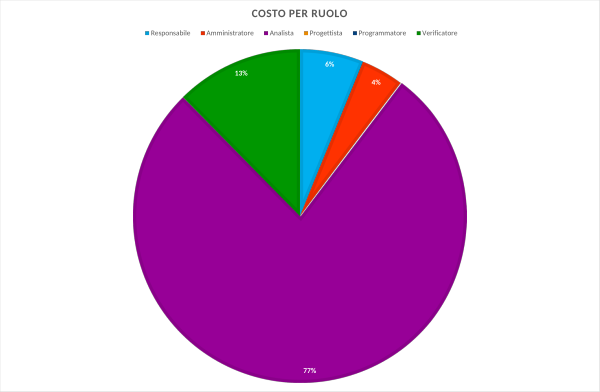
\includegraphics{img_peconomico/AD_CR.png}}
	\caption{Costi per ruolo, fase di \AD}
\end{figure}

\subsection{\PA}
Nella fase di \PA le ore sono suddivise nel modo seguente:
\begin{table}[H]
	\centering
	\begin{tabular}{|c|c|c|}
		\hline
		\textbf{Ruolo} &
		\textbf{Ore} &
		\textbf{Costo} \\
		\hline
		Responsabile & 8 & 240\\
		\hline
		Amministratore & 6 & 120\\
		\hline
		Analista & 23 & 575\\
		\hline
		Progettista & 101 & 2222 \\
		\hline
		Programmatore & 0 & 0 \\
		\hline
		Verificatore & 55 & 825\\
		\hline
		\textbf{Totale} & \textbf{193} & \textbf{3982} \\
		\hline
	\end{tabular}
	\caption{Costo per ruolo, fase di \PA}
\end{table}

I seguenti grafici mostrano visivamente come abbiano influiranno i ruoli per ore e costi nella fase di \PA.
\begin{figure}[H]
	\centering
	\scalebox{0.6}{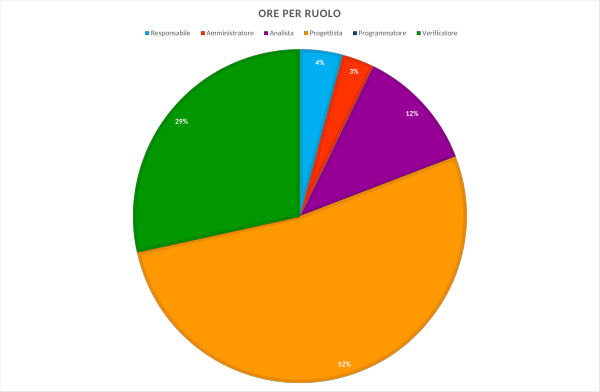
\includegraphics{img_peconomico/PA_OR.png}}
	\caption{Ore per ruoli, fase di \PA}
\end{figure}
\begin{figure}[H]
	\centering
	\scalebox{0.6}{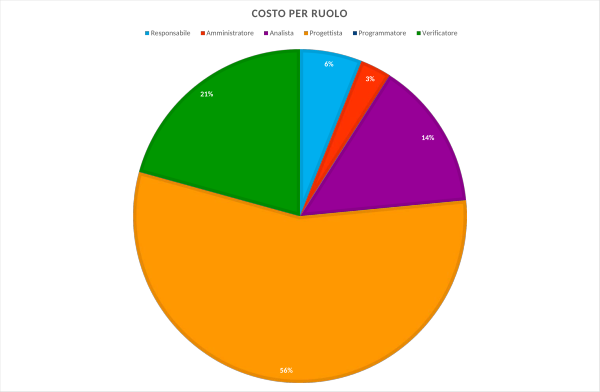
\includegraphics{img_peconomico/PA_CR.png}}
	\caption{Costi per ruolo, fase di \PA}
\end{figure}

\subsection{\PD}
Nella fase di \PD le ore sono suddivise nel modo seguente:
\begin{table}[H]
	\centering
	\begin{tabular}{|c|c|c|}
		\hline
		\textbf{Ruolo} &
		\textbf{Ore} &
		\textbf{Costo} \\
		\hline
		Responsabile & 8 & 240 \\
		\hline
		Amministratore & 8 & 160 \\
		\hline
		Analista & 4 & 100\\
		\hline
		Progettista & 98 & 2156 \\
		\hline
		Programmatore & 0 & 0 \\
		\hline
		Verificatore & 36 & 540 \\
		\hline
		\textbf{Totale} & \textbf{154} & \textbf{3196} \\
		\hline
	\end{tabular}
	\caption{Costo per ruolo, fase di \PD}
\end{table}

I seguenti grafici mostrano visivamente come abbiano influiranno i ruoli per ore e costi nella fase di \PD.
\begin{figure}[H]
	\centering
	\scalebox{0.6}{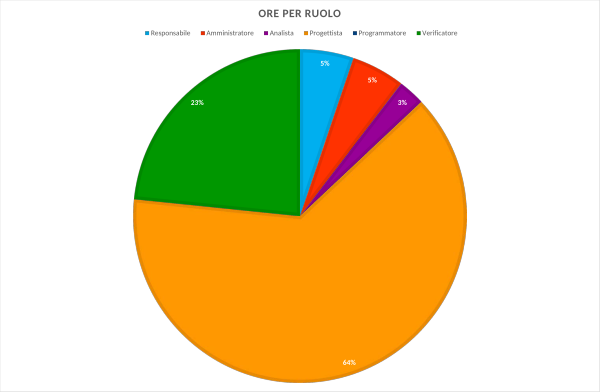
\includegraphics{img_peconomico/PD_OR.png}}
	\caption{Ore per ruoli, fase di \PD}
\end{figure}
\begin{figure}[H]
	\centering
	\scalebox{0.6}{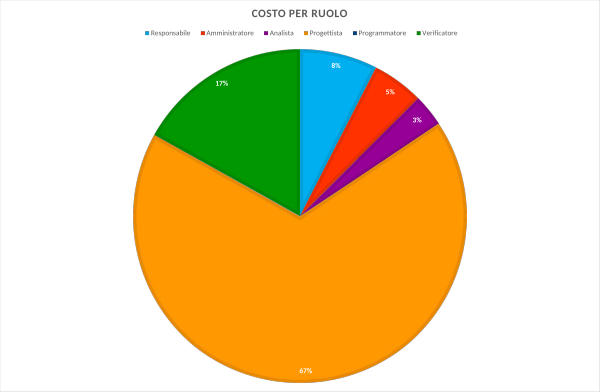
\includegraphics{img_peconomico/PD_CR.png}}
	\caption{Costi per ruolo, fase di \PD}
\end{figure}

\subsection{\Cod}
Nella fase di \Cod le ore sono suddivise nel modo seguente:
\begin{table}[H]
	\centering
	\begin{tabular}{|c|c|c|}
		\hline
		\textbf{Ruolo} &
		\textbf{Ore} &
		\textbf{Costo} \\
		\hline
		Responsabile & 9 & 270 \\
		\hline
		Amministratore & 4 & 80 \\
		\hline
		Analista & 0 & 0\\
		\hline
		Progettista & 15 & 330 \\
		\hline
		Programmatore & 144 & 2160 \\
		\hline
		Verificatore & 47 & 705 \\
		\hline
		\textbf{Totale} & \textbf{219} & \textbf{3545} \\
		\hline
	\end{tabular}
	\caption{Costo per ruolo, fase di \Cod}
\end{table}

I seguenti grafici mostrano visivamente come abbiano influiranno i ruoli per ore e costi nella fase di \Cod.
\begin{figure}[H]
	\centering
	\scalebox{0.6}{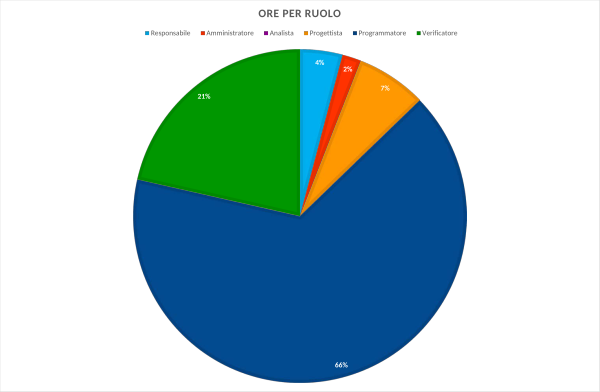
\includegraphics{img_peconomico/C_OR.png}}
	\caption{Ore per ruoli, fase di \Cod}
\end{figure}
\begin{figure}[H]
	\centering
	\scalebox{0.6}{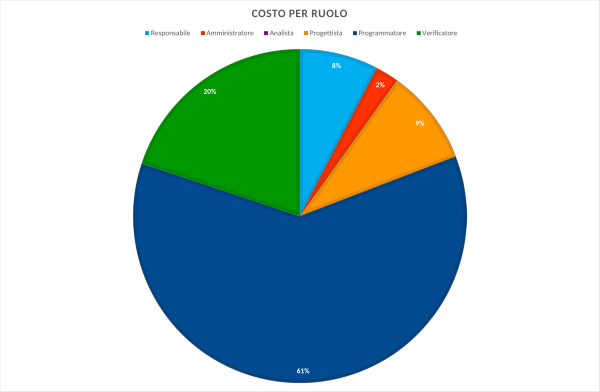
\includegraphics{img_peconomico/C_CR.png}}
	\caption{Costi per ruolo, fase di \Cod}
\end{figure}

\subsection{\VV}
Nella fase di \VV le ore sono suddivise nel modo seguente:
\begin{table}[H]
	\centering
	\begin{tabular}{|c|c|c|}
		\hline
		\textbf{Ruolo} &
		\textbf{Ore} &
		\textbf{Costo} \\
		\hline
		Responsabile & 10 & 300\\
		\hline
		Amministratore & 16 & 320\\
		\hline
		Analista & 0 & 0\\
		\hline
		Progettista & 13 & 286 \\
		\hline
		Programmatore & 12 & 180 \\
		\hline
		Verificatore & 83 & 1245\\
		\hline
		\textbf{Totale} & \textbf{134} & \textbf{2331} \\
		\hline
	\end{tabular}
	\caption{Costo per ruolo, fase di \VV}
\end{table}

I seguenti grafici mostrano visivamente come abbiano influiranno i ruoli per ore e costi nella fase di \VV.
\begin{figure}[H]
	\centering
	\scalebox{0.6}{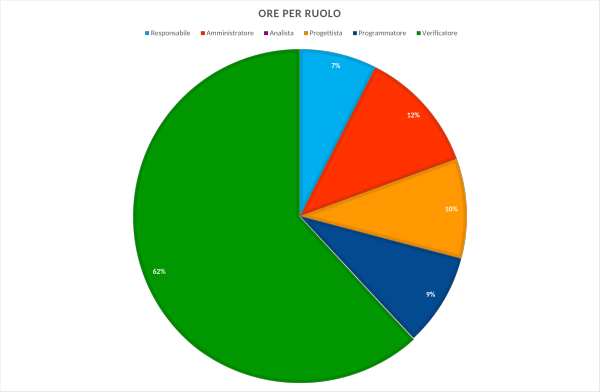
\includegraphics{img_peconomico/VV_OR.png}}
	\caption{Ore per ruolo, fase di \VV}
\end{figure}
\begin{figure}[H]
	\centering
	\scalebox{0.6}{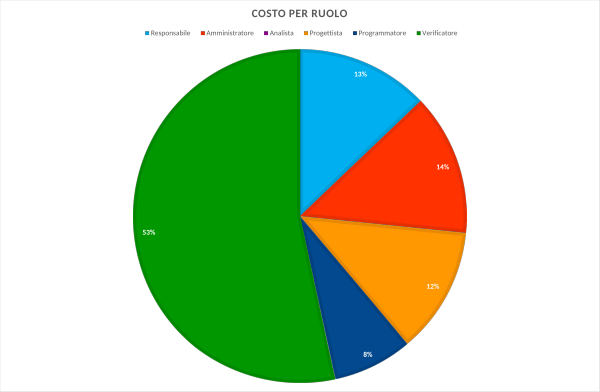
\includegraphics{img_peconomico/VV_CR.png}}
	\caption{Costi per ruolo, fase di \VV}
\end{figure}

\subsection{Totale}
\subsubsection{Ore totali con investimento}
Le ore complessive previste per ogni ruolo sono ripostate nella tabella sottsatante.
\begin{table}[H]
	\centering
	\begin{tabular}{|c|c|c|}
		\hline
		\textbf{Ruolo} &
		\textbf{Ore} &
		\textbf{Costo} \\
		\hline
		Responsabile & 66 & 1980\\
		\hline
		Amministratore & 64 & 1280\\
		\hline
		Analista & 132 & 3300\\
		\hline
		Progettista & 227 & 4994 \\
		\hline
		Programmatore & 156 & 2340 \\
		\hline
		Verificatore & 265 & 3975\\
		\hline
		\textbf{Totale} & \textbf{910} & \textbf{17869} \\
		\hline
	\end{tabular}
	\caption{Costo totale per ruolo}
\end{table}
I seguenti grafici mostrano visivamente come abbiano influiranno i ruoli per ore e costi nel progetto.
\begin{figure}[H]
	\centering
	\scalebox{0.6}{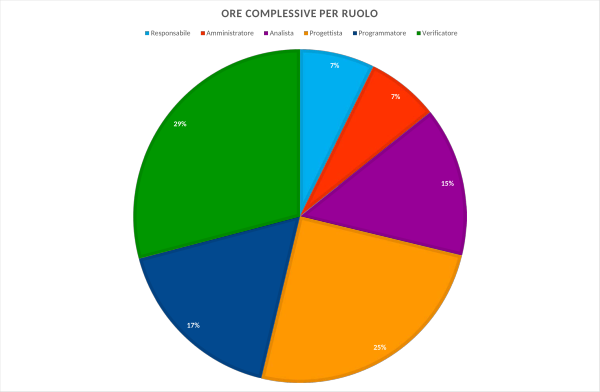
\includegraphics{img_peconomico/T_OR_C.png}}
	\caption{Ore totali per ruolo}
\end{figure}
\begin{figure}[H]
	\centering
	\scalebox{0.6}{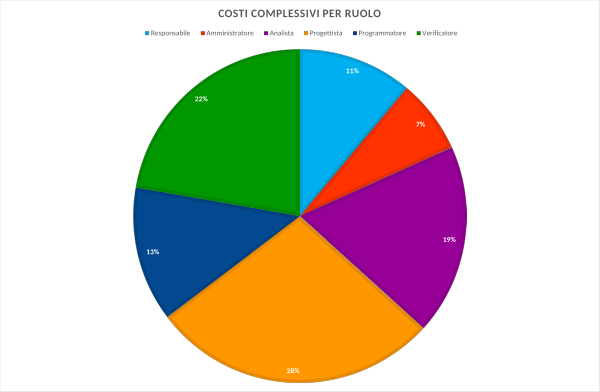
\includegraphics{img_peconomico/T_CR_C.png}}
	\caption{Costi totali per ruolo}
\end{figure}

\subsubsection{Ore rendicontate}
Le ore complessive rendicontate per ogni ruolo sono ripostate nella tabella sottsatante.
\begin{table}[H]
	\centering
	\begin{tabular}{|c|c|c|}
		\hline
		\textbf{Ruolo} &
		\textbf{Ore} &
		\textbf{Costo} \\
		\hline
		Responsabile & 35 & 1050\\
		\hline
		Amministratore & 34 & 680\\
		\hline
		Analista & 27 & 675\\
		\hline
		Progettista & 227 & 4994 \\
		\hline
		Programmatore & 156 & 2340 \\
		\hline
		Verificatore & 221 & 3315\\
		\hline
		\textbf{Totale} & \textbf{700} & \textbf{13054} \\
		\hline
	\end{tabular}
	\caption{Costo totale per ruolo}
\end{table}
I seguenti grafici mostrano visivamente come abbiano influiranno i ruoli per ore e costi nel progetto.
\begin{figure}[H]
	\centering
	\scalebox{0.6}{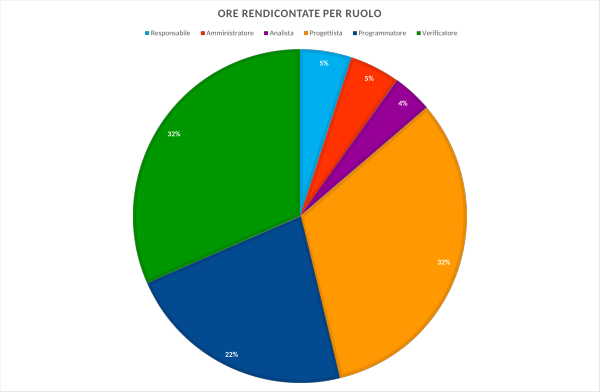
\includegraphics{img_peconomico/T_OR_R.png}}
	\caption{Ore totali per ruolo}
\end{figure}
\begin{figure}[H]
	\centering
	\scalebox{0.6}{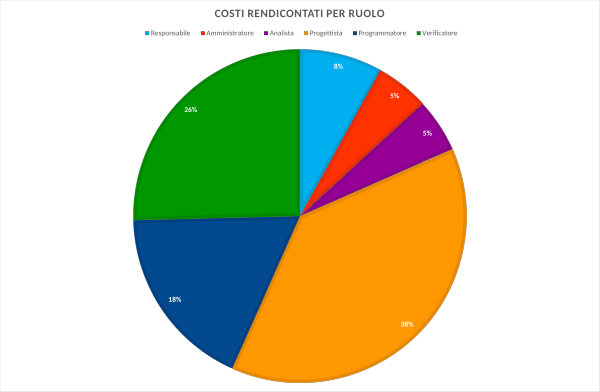
\includegraphics{img_peconomico/T_CR_R.png}}
	\caption{Costi totali per ruolo}
\end{figure}





